\subsection{Phân tích phương sai một nhân tố (Single-factor ANOVA)}


Nhóm gọi:
\begin{itemize}
    \item Y: là một biến phụ thuộc (có tính liên tục).
    \item X: là một biến nhân tố hay biến giải thích (có tính phân loại).
\end{itemize}

Yêu cầu:
\begin{itemize}
    Đánh giá xem biến nhân tố X có ảnh hưởng đến biến phụ thuộc Y hay không?
\end{itemize}
Giả thuyết:
  \[
  H_{0}: \mu_{1} = \mu_{2} = \mu_{3} = \dots = \mu_{n}
  \]
  \[
  H_{1}: \exists i, j \text{ sao cho } \mu_{i} \neq \mu_{j}
  \]

- Đọc dữ liệu từ file và đưa ra bảng dữ liệu:
%   sxtk = read.csv("/Users/Windows10/Documents/Zalo Received Files/dirty_data.csv", header=T)
%   attach(sxtk)

%- Bảng dữ liệu:
% freq_table <- dt[,.N, by=coupon_discount]
% colnames(freq_table) <- c("coupon_discount", "count")

\begin{figure}[!htbp]
    \centering
    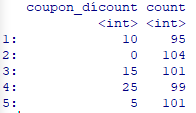
\includegraphics[width=0.4\linewidth]{graphics/5.3.1.png}
    \caption{Số lượng mặt hàng (count) theo từng loại chiết khấu (coupon\_discount)}
\end{figure}

Như trên Hình 1, chỉ có 5 giá trị của coupon_discount là : 0, 5, 10, 15, 25. Nhóm sẽ kiểm định xem, việc các mốc chiết khấu này sẽ ảnh hưởng như thế nào đến giá của các mặt hàng (order_price) bằng phương pháp phân tích phương sai ANOVA mà nhóm đã thảo luận và đề xuất sử dụng. Dưới đây là phân tích phương sai ANOVA cho mẫu thống kê ( hàm phân tích đã được tích hợp sẵn trong R) :
